\documentclass[12pt,letterpaper]{article}
\usepackage{iwona}
\usepackage{setspace}
\usepackage[utf8]{inputenc}
\usepackage[portuguese]{babel}
\usepackage[version=3]{mhchem}
\usepackage[journal=jacs]{chemstyle}
\usepackage[affil-it]{authblk} 
\usepackage{tikz}
\usepackage{hyperref}
\usepackage{cite}  
\usepackage{tabularx}
\usepackage{indentfirst}

\usepackage[left=3cm,right=2cm,top=1.7cm,bottom=1.7cm]{geometry}


%======================================================================
  
  \begin{document}
\onehalfspacing 
\thispagestyle{empty}

\begin{center}
\vspace{0.2cm}

\hrulefill

\textbf{UNIVERSIDADE FEDERAL DE ALAGOAS}\\
\textbf{PRÓ-REITORIA DE PESQUISA E PÓS-GRADUAÇÃO}\\
COORDENAÇÃO DE PESQUISA

\hrulefill

\vspace{0.5cm}

PROGRAMA INSTITUCIONAL DE BOLSAS DE INICIAÇÃO\\ CIENTÍFICA -- PIBIC CNPq/UFAL/FAPEAL

\vspace{1.0cm}

\textbf{\textit{\Large{RELATÓRIO FINAL \\ (2018 -- 2019)}}}\\

\vspace{1.2cm}

\textbf{TÍTULO DO PROJETO DE PESQUISA:}

\underline{Aplicações Inovadoras da Teoria da Informação no Processamento e Análise de}

\underline{Imagens e Sinais}

\vspace{0.6cm}

\textbf{TÍTULO DO PLANO DE TRABALHO:}

\underline{Visualização e Processamento de Grandes Imagens SAR}

\end{center}

\textbf{\underline{NOME DO ORIENTADOR:}} Alejandro César Frery 

\vspace{0.4cm}

\textbf{\underline{NOME DO BOLSISTA:}} Danilo Fernandes Costa

\vspace{1cm}

\begin{table}[!h]
\begin{center}
\begin{tabularx}{\textwidth}{|X|X|X|X|}
\hline                              
\hspace{1.3cm} X & Bolsista CNPq &  &Bolsista FAPEAL\\
\hline             
& Bolsista UFAL &  &Colaborador\\
\hline     
\end{tabularx}
\end{center}
\end{table}

GRANDE ÁREA DO CONHECIMENTO (CNPq): Ciências  Exatas  e  da  Terra

SUB-ÁREA DO CONHECIMENTO (CNPq) : Processamento Grafico (\textit{Graphics})  

\vspace*{0.8cm}

\begin{center}

Maceió - AL, 15/08/2019

\end{center}

%=================================================================
  
  \newpage
\section*{\centering \textbf{RESUMO}} % (Máximo 1 página – Sem parágrafos) 

Houve um significativo avanço nos últimos anos na obtenção de novos métodos para a extração de informação a partir de sinais e imagens empregando técnicas oriundas da Teoria da Informação. Essas técnicas empregam duas abordagens. A primeira consiste em calcular diversas formas de entropia através de modelos analíticos; essas entropias são atributos descritores, e podem ser usados para calcular o contraste entre dois sinais, isto é, quão diferentes eles são. A segunda abordagem emprega dois sinais e seus modelos analíticos, e calcula diversas medidas de dissimilaridade entre eles. Tanto os contrastes oriundos de diferenças de entropias quanto as medidas de dissimilaridade podem ser transformados em testes estatísticos com propriedades assintóticas conhecidas tornando-se, assim, em poderosas ferramentas para a realização de comparações e para a tomada de decisões. Este projeto irá concentrar-se na aplicação dessas ferramentas em problemas relevantes de processamento e análise de sinais e imagens. Os principais problemas a serem abordados são na área de processamento e análise de imagens, em particular de imagens de radar de abertura sintética polarimétrico (SAR \textit{Synthetic Aperture Radar} e PolSAR -- \textit{Polarimetric Synthetic Aperture Radar}) e de séries temporais. Faremos a proposta de novos filtros, classificadores, segmentadores e detetores de mudança para as primeiras, e de novos descritores e quantificadores de mudança para as segundas. Este projeto irá ainda fazer avanços teóricos. Os resultados conhecidos para os testes estatísticos são válidos apenas no sentido assintótico e quando são empregados estimadores de máxima verossimilhança. Estudaremos extensões para os casos de amostras finitas e outros tipos de estimadores (baseados no princípio da analogia, robustos, e não-paramétricos, dentre outros).

\textbf{Palavras-chave: Teoria da Informação; Imagens SAR; Séries Temporais} 
%=========================================================
  
  \newpage
\section*{\centering \textbf{INTRODUÇÃO E OBJETIVOS}} %(Máximo 1 página)

A primeira abordagem citada acima parte do pressuposto que há dados disponíveis em uma amostra $z = (z1, . . . , zn)$ e um modelo para eles $D(\theta)$, com $\theta \in \Theta \subset R ^ p$ o espaço paramétrico. O modelo $D(\theta)$ induz uma única forma de entropia $H$, e para calcularmos uma estimativa da entropia $H(\theta)$ a partir da amostra $z$ é necessário estimar o parâmetro $\theta$. O modelo que nos interessa para dados SAR e a distribuição $G^0$, proposta por Frery, Muller, Yanasse \& Sant’Anna (1997). Conhecemos várias técnicas para estimar $\theta$ a partir de $z$: momentos fracionários (Mejail, Jacobo-Berlles, Frery \& Bustos, 2003), máxima verossimilhança e máxima verossimilhança iterada (Frery, Cribari-Neto \& Souza, 2004), estimadores robustos (Bustos, Lucini \& Frery, 2002; Allende, Frery, Galbiati \& Pizarro, 2006), estimadores de kernel (Gambini, Cassetti, Lucini \& Frery, 2015), log-momentos e estatísticas de ordem superior (Deng \& López-Martínez, 2016). Além dessas tecnicas de estimação, há métodos para melhorar as estimativas, notadamente baseados em reamostragem (Cribari-Neto, Frery \& Silva, 2002) e em correções analíticas (Silva, Cribari-Neto \& Frery, 2008). Cada uma dessas técnicas está associada a diferentes algoritmos, e resulta mais adequada para uma diversidade de situações (pequenas amostras, suspeita de contaminação, etc.). O desafio deste projeto é construir uma unica rotina que seja capaz de identificar qual é a melhor estratégia de estimação para a amostra de entrada, e que retorne uma estimativa de $\theta$ com a menor intervenção possível por parte do usuário.

A segunda abordagem consiste no uso da técnica de simbolização de Bandt \& Pompe (2002) para análise de séries temporais. Essa técnica consiste em transformar vetores de tamanho \textit{D} em padroes ordinais de forma nao-paramétrica, em formar um histograma de ocorrência dos \textit{D!} padroes possíveis, e em calcular descritores baseados em Teoria da Informação (Entropias, Distâncias Estocásticas, Complexidade Estatística) a partir desse histograma. Esses descritores passam a caracterizar a série temporal. Trata-se de uma técnica poderosa que tem sido aplicada em uma diversidade de situações (ver Rosso, Ospina \& Frery, 2016, e as referências aí citadas), mas que requer que não haja valores repetidos na série original.

Este projeto visa desenvolver tecnicas de imputação dos padrões não observados por causa da ocorrência de repetição de dados. Ambas abordagens utilizam de forma intensa conceitos e ferramentas de Teoria da Informação e de Geometria da Informação.

%=========================================================
  
\newpage
\section*{\centering \textbf{METODOLOGIA}} %(Máximo 2  páginas)
%Etapas do plano de trabalho
A metodologia de ambas iniciativas consiste em
\begin{enumerate}
\item Conhecer a literatura fundamental sobre cada tema.
\item Desenvolver protótipos de software.
\item Submeter os protótipos a testes de acurácia, precisão e robustez com dados de propriedades conhecidas.
\item Analisar métodos para decidir quais são as técnicas mais adequadas para cada situação, em função apenas dos dados de entrada.
\item Analisar a forma de trabalho de usuarios finais.
\item Integrar as soluções em ferramentas de uso amigável para esses usuários.
\item Validar os resultados na prática.
\end{enumerate}

%=========================================================
  
\newpage
\section*{\centering \textbf{RESULTADOS E DISCUSSÕES}} %(máximo 4 páginas)
O período designado ao projeto foi consolidado sobre os constantes avanços teóricos em virtude da busca de literatura referente às temáticas que permeiam o escopo da pesquisa, onde foram buscados diversos artigos de qualidade escritos por autores referência na temática em questão.

O conhecimento teórico adquirido possibilitou a implementação de funções em linguagem R que viriam a integrar a biblioteca proposta pelo projeto de pesquisa dedicada ao processamento de grandes imagens PolSAR. No desenvolvimento dessas, explorou-se ao máximo os recursos disponibilizados pela biblioteca raster. A justificativa para a utilização desta é que a mesma visa prover um ambiente para a análise de dados geográficos -- modalidade que inclui dados SAR -- e fornece mecanismos para o processamento de volume de dados que excedem a capacidade da memória principal do computador. Dentre esses mecanismos, a leitura e escrita de segmentos específicos do arquivo em formato matricial foram essenciais, visto que os arquivos referentes a este tipo imagens PolSAR recorrentemente são grandes o suficiente em relação à memória principal para produzir um gargalo no processamento.

A funcionalidade mais basilar implementada foi a visualização dos dados PolSAR, a qual consiste na realização de operações matemáticas sobre estes que resultam em conjunto três valores reais para cada \textit{pixel} da imagem os quais representam uma cor. Os métodos para a visualização implementadas foram através da projeção direta no espaço das cores e da decomposição de Pauli. Ambas permitem a observação da estratura física da região imageada, mas a segunda atribui tonalidades de verde às regiões encobertas por vegetação. 

Uma outra funcionalidade desenvolvida foi um filtro baseado no coeficiente de variação cujo produto é uma outra imagem na qual os dados referentes a regiões homogêneas apresentam um comportamento estatístico modelável por uma distribuição de probabilidade conhecida.



%=========================================================
  
  \newpage
\section*{\centering \textbf{CONCLUSÕES}} %(máximo 2  páginas)



%=========================================================
  
  \newpage
%REFERÊNCIAS BIBLIOGRÁFICAS (máximo 2  páginas)

\bibliographystyle{unsrt}
\bibliography{references}

%=========================================================
  
  \newpage

\section*{\centering \textbf{PLANO DE TRABALHO INDIVIDUAL E DIFERENCIADO DO BOLSISTA OU COLABORADOR}} %(igual projeto original) 2 páginas

\textbf{TÍTULO DO PLANO DE TRABALHO:} \underline{Visualização e Processamento de Grandes Imagens SAR}

\textbf{Objetivos do trabalho da estudante:} Desenvolver tecnicas de visualização e processamento de grandes imagens SAR. Montar uma biblioteca de imagens SAR gratuita. Montar uma biblioteca de amostras de imagens SAR.\\

\textbf{Metodologia correspondente:}

\textbf{Atividade 1:} Conhecer tecnicas de visualização e de processamento de grandes imagens SAR.

\textbf{Atividade 2:} Aprender o uso da plataforma \textit{R}.

\textbf{Atividade 3:} Conhecer técnicas de projeto e implementação de software científico usando \textit{R}.

\textbf{Atividade 4:} Desenvolver prototipos de algoritmos de visualização e de processamento de imagens SAR.

\textbf{Atividade 5:} Aplicar as técnicas desenvolvidas a conjuntos de dados de propriedades conhecidas.

\textbf{Atividade 6:} Integrar as técnicas desenvolvidas em uma plataforma de produção.\\

\begin{figure}[H]
\begin{center}
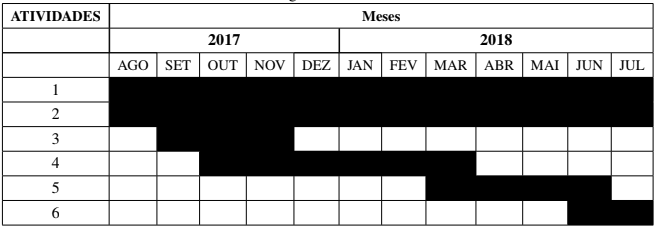
\includegraphics[width=0.95\columnwidth]{cronograma}
\end{center}
\end{figure}

\end{document}